\section{Genetic drift and Neutral alleles}



\subsection{The fixation of neutral alleles}
It is very unlikely that a rare neutral allele accidentally drifts up
to fixation, it is much more likely that such an allele is eventually
lost from the population. However, there is a large and constant influx of
rare alleles into the population due to mutation, so even if it is very
unlikely that an individual allele fixes within the population, some
neutral alleles will fix.  \\

%We'll first consider the probability that a neutral allele fixes
%within the population, starting from it just enters a diploid
%population as a newly mutated allele at frequency $1/(2N)$.

%so for an allele to be fixed in the population it
%must have been that allele


\paragraph{Probability of the eventual fixation of a neutral allele.} An allele which reaches fixation within a population, is an ancestor to
the entire population. In a particular generation there can be only single
allele that all other alleles at the locus in  later generation can claim as an
ancestor. As at a neutral locus all of our alleles are exchangeable, as
they have no effect on the number of descendents an individual
leaves, so any allele is equally likely to be the ancestor of the
entire population.  In a diploid population size of size $N$, there are $2N$
alleles all of which are equally likely to be the ancestor of the
entire population at some later time point. So if our allele is present in a single copy, the chance that
is the ancestor to the entire population in some future generation is
$1/(2N)$, i.e. the chance our neutral allele is eventually fixed is
$1/(2N)$.\\

More generally if our neutral allele is present in $i$ copies in the
population, of $2N$ alleles, the probability that this allele is fixed
is $i/(2N)$. I.e. the probability that a neutral allele is eventually
fixed is simply given by its frequency ($p$) in the population.
We can also derive this result by letting $Ns \rightarrow
0$ in eqn. \eqref{eqn:prob_fixed}.

\paragraph{Rate of substitution of neutral alleles.}

A substitution between populations that do not exchange gene flow is
simply a fixation event within one population. The rate of
substitution is therefore the rate at which new alleles fix in the
population, so that the long-term substitution rate is the rate at
which mutations arise that will eventually become fixed within our population.\\

Assume that there are two classes of mutational changes that can occur with a
region, highly deleterious mutations and neutral mutations. A fraction
$C$ of all mutational changes are highly deleterious, and can not
possibly contribute to substitution nor polymorphism (i.e. $Ns \gg 1$).
While a fraction $1-C$ are neutral. If our mutation rate is $\mu$ per
transmitted allele per generation, then a total of $2N \mu (1-C)$
neutral mutations enter our population each generation.\\

Each of these neutral mutations has a $1/(2N)$ probability chance of
eventually becoming fixed in the population. Therefore, the rate at
which neutral mutations arise that eventually become fixed within our
population is  
\begin{equation}
2N\mu(1-C)\frac{1}{2N} = \mu(1-C)
\end{equation}
thus the rate of substitution under a model where newly arising alleles are either
highly deleterious or neutral, is simply given by the mutation rate
towards neutral alleles, i.e. $\mu(1-C)$.\\

Consider a pair of species have diverged for $T$ generations, i.e. orthologous sequences shared between the species last shared a common ancestor $T$ generations ago. If they have maintained a constant $\mu$ over that time, will have accumulated an average of
\begin{equation}
2\mu(1-C)T
\end{equation}
neutral substitutions. This assumes that $T$ is a lot longer than the time it
takes to fix a neutral allele, such that the total number of 
alleles introduced into the population that will eventually fix is the
total number of substitutions. We'll see below that a neutral allele
takes on average $4N$ generations to fix from its introduction into
the population.\\

This is a really pretty result as the population size has completely
canceled out of the neutral substitution rate. However, there is
another way to see this in a more straightward way. If I look at a
sequence in me compared to say a particular chimp, I'm looking at the mutations
that have occurred in both of our germlines since they parted ways $T$
generations ago. Since neutral alleles do not alter the probability
of their transmission to the next generation, we are simply looking at
the mutations that have occurred in $2T$ generations worth of
transmissions. Thus the average number of neutral mutational
differences separating our pair of species is simply $2\mu (1-C) T$.\\


\subsection{The Coalescent and patterns of neutral diversity}

\paragraph{Pairwise Coalescent time distribution and the number of
 pairwise differences.}
Thinking back to our calculations we made about the loss of neutral heterozygosity
and equilibrium levels of diversity (in Sections \ref{LossofHet} and \ref{DriftMutationBalance}), you'll note that we could first specify
what generation a pair of sequences coalesce in, and then calculate
some properties of heterozygosity based on that. That's because neutral
mutations do not affect the probability that an individual transmits
that allele, so don't affect the way in which we can trace ancestral lineages
back. \\

As such it will often be helpful to consider the time to the common
ancestor of a pair of sequences, and then think of the impact of that
on patterns of diversity. See Figure \ref{fig:Coalescent_simulation}
for an example of this. The probability that a pair of alleles
have failed to coalesce in $t$ generations and then coalesce in the
$t+1$ generation back is
\begin{equation}
\frac{1}{2N} (1- \frac{1}{2N} )^{t} \approx \frac{1}{2N} e^{-t/(2N)} \label{eqn:coal_time_dist}
\end{equation}
thus the coalescent time of a pair of sequences ($T_2$) is
approximately exponentially distributed with a rate $1/(2N)$. We'll denote that by
saying that $T_2 \sim Exp \left( 1/(2N) \right)$. The mean coalescent
time of a pair of a pair of alleles is $2N$ generations\\


\begin{figure}
\begin{center}
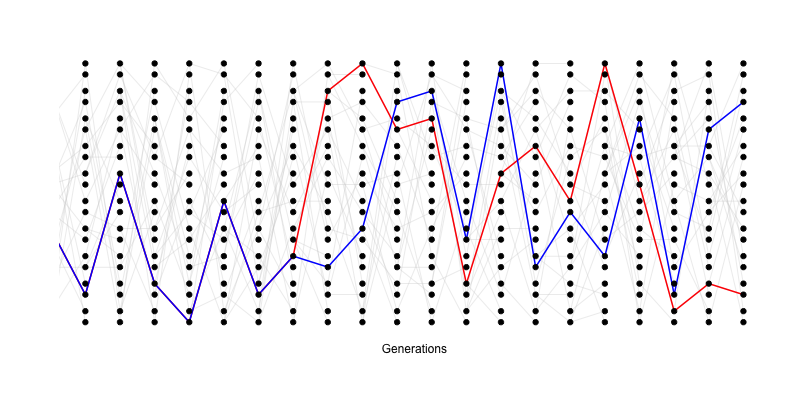
\includegraphics[width=\textwidth]{figures/Coalescent.png}
\end{center}
\caption{A simple simulation of the coalescent process. The simulation
  consists of a diploid population of 10 individuals (20 alleles). In
  each generation, each individual is equally likely to be the parent
  of an offspring (and the allele transmitted is indicated by a light
  grey line).  We track a
  pair of alleles, chosen in the present day, back 14 generations
  untill they find a common ancestor.} \label{fig:Coalescent_simulation}
\end{figure}



Conditional on a pair of alleles coalescing $t$ generations ago
there are $2t$ generations in which a mutation could occur. Thus the
probability of our pair of alleles are separated by $j$ mutations
since they last shared a common ancestor is
\begin{equation}
P(j | T_2 = t ) = {2t \choose j} \mu^{j} (1-\mu)^{2t-j}
\end{equation}
i.e. mutations happen in $j$ generations, and do not happen in $2t-j$
generations (with ${2t \choose j}$ ways this can possibly
happen). Assuming that $\mu \ll 1$, and that $2t-j \approx 2t$ then we
can approximate the probability that we have $j$ mutations as a
Poisson distribution
\begin{equation}
P(j | T_2 = t ) = \frac{ (2 \mu t )^{j} e^{-2\mu t}}{j!}
\end{equation}
i.e. a Poisson with mean $2\mu t $. \\

As our expected coalescent time is $2N$ generations, the expected
number of mutations separating two alleles drawn at random from the
population is
\begin{equation}
\E(j) = 4N\mu = \theta
\end{equation}
We'll assume that mutations never happen at the same site twice,
i.e. no multiple hits, such that we get to see all of the mutation events that separate our pair
of sequences (we'll call this the infinitely-many-sites assumption,
which should be fine if $N\mu_{BP} \ll 1$). Thus the number of
mutations between a pair of sites is the observed number of
differences between a pair of sequences. \\


We'll denote the observed number of pairwise differences at putatively
neutral sites separating a
pair of sequences as $\pi$ (we usually average this over a number of
pairs of sequences for a region). So we can estimate of
$\theta$ from $\pi$, $\widehat{\theta}_{\pi}$ by setting $\widehat{\theta}_{\pi}=\pi$.
If we have an independent
estimate of $\mu$, then from setting $\pi = \widehat{\theta}_{\pi} = 4N\mu$ we can obtain an
estimate of the population size $N$ that is consistent with our levels
of neutral polymorphism.



\subsection{The coalescent process of a sample of alleles.}

Usually we are not just interested pairs of alleles, or the
average pairwise diversity, we are interested in the properties of
diversity in samples of a number of alleles drawn from the population.  
To allow for this instead of just following a pair of lineages back until they
coalesce, we can follow the history of a sample of alleles back
through the population.

Consider first sampling three alleles at random from the
population. The probability that all three alleles choose exactly the
same ancestral allele one generation back is $1/(2N)^2$. If $N$ is
reasonably large then this is a very small probability. As such it is
very unlikely that our three alleles coalesce at once, a in a moment
we'll see that it is safe to ingnore such unlikely events. \\

The
probability that a specific pair of alleles find a common ancestor in
the preceding generation is still $1/(2N)$. There are three possible
pairs of alleles so the probability that no pair finds a common
ancestor is
\begin{equation}
\left(1-\frac{1}{(2N)} \right)^3 \approx \left( 1- \frac{3}{2N} \right)
\end{equation}
in making this approximation we are multiplying out the right hand-side
and ignoring terms of $1/N^2$ and higher. See
Figure \ref{fig:Coalescent_simulation_3} for a random realization of this process. \\


\begin{figure}
\begin{center}
  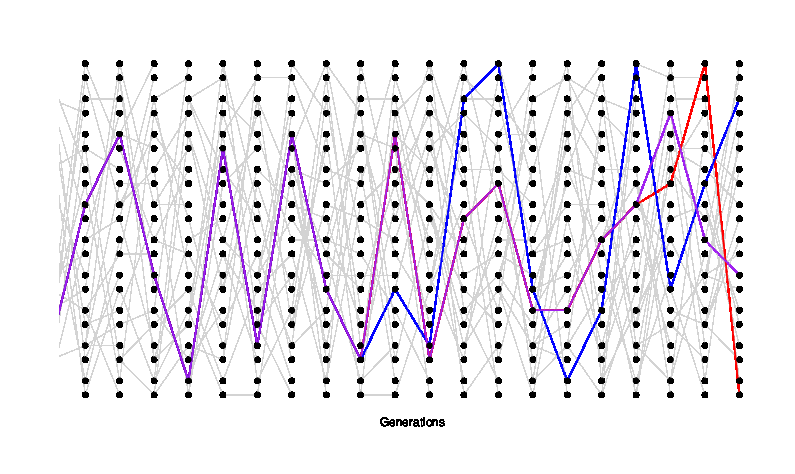
\includegraphics[width = \textwidth]{figures/Coalescent_3.png}
\end{center}
\caption{A simple simulation of the coalescent process for three
  lineages. We track the ancestry of 
  three modern-day alleles, the first pair (blue and purple) coalesce four generations back 
  their are then two independent lineages we are tracking, this pair
  then coalesces twelve generations in the past. Note that different
  random realizations of this process will differ from each other a lot.} \label{fig:Coalescent_simulation_3}
\end{figure}


More generally when we sample $i$ alleles there are ${i \choose
 2}$ pairs, i.e. $i(i-1)/2$ pairs, thus the probability that no pair
of alleles coalesces in the preceding generation is
\begin{equation}
\left(1-\frac{1}{(2N)} \right)^{{i \choose
 2}} \approx \left( 1- \frac{{i \choose
 2}}{2N}\right)
\end{equation}
while the probability of any pair coalescing is $\approx \frac{{i \choose
 2}}{2N}$.\\

We can ignore the possibility of more than pairs of alleles (e.g. tripletons) simultaneously
coalescing at once as terms of $1/N^2$ and higher can
be ignored as they are vanishingly rare. Obviously there are in reasonable sample sizes there are
many more triples (${i \choose 3}$), and higher order combinations, than pairs
(${i \choose 2}$) but if $i \ll N$ then we are safe to
ignore these terms.

When there are $i$ alleles the probability that we wait until the
$t+1$ generation before
any pair of alleles coalesce is
\begin{equation}
 \frac{{i \choose
 2}}{2N}\left( 1- \frac{{i \choose
 2}}{2N}\right)^{t} \approx  \frac{{i \choose
 2}}{2N} \exp \left( - \frac{{i \choose
 2}}{2N} t \right)
\end{equation}
thus the waiting time $T_i$ to the first coalescent event in a sample
of $i$ alleles is exponentially distributed with rate $\frac{{i \choose
 2}}{2N}$, i.e. $T_i \sim Exp\left(\frac{{i \choose
 2}}{2N} \right)$. The mean waiting time till any of pair within our
sample to coalesce is $2N/{i \choose
 2}$.\\

When a pair of alleles first find a common ancestral allele some
number of generations back further into the past we only have to keep
track of that common ancestral allele for the pair. Thus when a pair
of alleles in our sample of $i$ alleles coalesce, we then switch to
having to follow $i-1$ alleles back. Then when a pair of these $i-1$
alleles coalesce, we then have to follow $i-2$ alleles back. This
process continues until we coalesce back to a sample of two, and from
there to a single most recent common ancestor (MRCA).\\


To simulate a coalescent genealogy at a locus for a sample of $n$ alleles we therefore simply follow this
algorithm
\begin{enumerate}
\item set $i=n$.
\item We simulate a random variable to be the time $t_i$ to the next coalescent event from $t_i \sim
 Exp\left(\frac{{i \choose
 2}}{2N} \right)$
\item choose a pair of alleles to coalesce at random from all possible
 pairs.
\item set $i=i-1$
\item continue looping of steps 1-3 until $i=1$ i.e. the most recent
 common ancestor of the sample is found.
\end{enumerate}
by following this algorithm we are generating realizations of the
genealogy of our sample. \\

We will first consider the time to the most recent common ancestor of
the entire sample ($T_{MRCA}$). This is
\begin{equation}
T_{MRCA} = \sum_{i=n}^2 T_i
\end{equation}
generations back. As our coalescent times for different $i$ are independent, the expected time to the most recent common ancestor
is
\begin{equation}
\E(T_{MRCA}) = \sum_{i=n}^2 \E(T_i) = \sum_{i=n}^2  2N/{i \choose
 2}
\end{equation}
using the fact that $\frac{1}{i(i-1)}=\frac{1}{i-1} - \frac{1}{i}$ with a bit of
rearrangement we can rewrite this is
\begin{equation}
\E(T_{MRCA}) = 4N\left(1- \frac{1}{n} \right)
\end{equation}
so the average $T_{MRCA}$ scales linearly with population
size. Interestingly, as we move to larger and larger samples (i.e. $n \gg 1$) the average
time to the most recent common ancestor is converging on $4N$. What's
happening here is that in large samples our lineages typically coalesce rapidly
at the start and very soon coalesce down to a much smaller number of
lineages.   \\

Above we argued that a mutation is only becomes a fixed difference if
it is lucky enough to be the
ancestor of the entire population. As we saw above this occurs with
probability $1/(2N)$. How long does is take on average for such an
allele to fix within our population. We've just seen that it
takes $4N$ generations for a large sample of alleles to all trace
their ancestry back to a single most recent common
ancestor. Thus it must take roughly $4N$ generations for a neutral
allele present in a single copy within the the population to the
ancestor of all alleles within our population. This argument can be
made more precise, but in general we would still find that it takes
$\approx 4N$ generations for a neutral allele to go from its
introduction to fixation with the population.   \\


%%point about the fixation time of a neutral allele


The total amount of time in the genealogy ($T_{tot}$)
\begin{equation}
T_{tot} = \sum_{i=n}^2 iT_i
\end{equation}
as when there are $i$ lineages each contributes a time $T_i$ to the
total time. Taking the expectation of the total time in the genealogy
\begin{equation}
\E(T_{tot}) = \sum_{i=n}^2 i \frac{2N}{{i \choose
 2} } = \sum_{i=n}^2 \frac{4N}{i -1} =\sum_{i=n-1}^1 \frac{4N}{i}
\end{equation}
so our expected total amount of time in the genealogy scales linearly
with our population size. Our expected total amount of time is also
increasing with sample size but is doing so very slowly. To see this
more carefully we can see that for large $n$
\begin{equation}
\E(T_{tot}) = \sum_{i=n-1}^1 \frac{4N}{i} \approx 4N \int_1^n \frac{1}{i} di
= 4N \log(n-1)
\end{equation}
here we are approximating our sum by an integral, which will work for
large $n$. So our expected total amount of time in the genealogy
is growing with $n$ but it is doing so very slowly. This again follows
from the fact that in large samples the initial coalescence usually
happens very rapidly, so that extra samples adds little to the total
amount of time in the tree. \\


We saw above that the number of mutational differences between a pair
of alleles that coalescence $T_2$ generations ago was Poisson with a
mean of $2 \mu T_2$. A mutation that occurs on any branch of our
genealogy will cause a segregating polymorphism in the sample
(making our infinitely-many-sites assumption). Thus if the total time
in the genealogy is $T_{tot}$ there is $T_{tot}$
generations for mutations. So the total number of mutations
segregating in our sample ($S$) is Poisson with mean $\mu T_{tot}$. Thus the
expected number of segregting  in history a sample of size $n$ is
\begin{equation}
\E(S) = \mu \E(T_{tot}) = \sum_{i=n-1}^1 \frac{4N\mu }{i} = \theta
\sum_{i=n-1}^1 \frac{1}{i}
\end{equation}
Thus we can use this formula to derive another estimate of the
population scaled mutation rate, by setting our observed number of
segregating sites in a sample ($S$) equal to this expectation. We'll call this estimator $\widehat{\theta}_W$
\begin{equation}
\widehat{\theta}_W =\frac{ S}{\sum_{i=n-1}^1 \frac{1}{i}}  
\end{equation}
this estimator was devised by Watterson, hence the $W$.


\subsection{Comparing polymorphism and divergence}


\subsection{Deviations from the constant population model.}
We've seen previously that changes in our population size can be
captured by an effective population size. However, this will only be a
useful measure if population sizes vary rapidly enough, that the
harmonic mean effective population size over short time periods ($\ll
N_e$ generations) is representative of the effective population size averaged over
longer time periods. If this is not the case there is no one effective
population size, as we can not approximate our rate of drift by a
single constant population. Furthermore, we've ignored the effect of
population structure and selection which will violate our modeling
assumptions. \\

We can hope to detect violations from our constant population size
neutral model, by comparing aspects of our dataset to their expectations
and distributions under our neutral model. \\

For example we have devised two estimates of $\theta$,
$\widehat{\theta_{\pi}}$ and $\widehat{\theta_{W}}$, using
expectations of different aspects of our data (pairwise diversity and
number of segregating sites respectively). Under our constant neutral
model if we have sufficient data those two estimates should be
equal to each other on average. But if there's some violation of our model they might not
be. So one test statistic might be to take
\begin{equation}
D = \widehat{\theta_{\pi}} - \widehat{\theta_{W}}
\end{equation}
which will be zero in expectation if our data was generated by a
neutral constant population model.




\newpage
